\section{Resultados}
\label{sec:resultados}

La Tabla~\ref{tab:f1} reproduce los 12 casos de la Tabla~3 del artículo. La columna \textit{noKD} es el F1 absoluto del mBERT ajustado sin destilación; las tres restantes son diferencias en puntos de F1 frente a ese baseline. El artículo no publica el F1 absoluto de los modelos destilados, así que la comparación se hace sobre deltas.

\begin{table}[H]
\centering
\caption{F1 del baseline sin destilación y diferencia de cada profesor.}
\label{tab:f1}
\small
\setlength{\tabcolsep}{4pt}
\begin{tabular}{@{}llrrrr@{}}
\toprule
Lengua & Datos & \textit{noKD} & $B_p$ & $B_{ft}$ & $mB_{ft}$ \\
\midrule
Español & 10\,\%  & $73{,}46$ & $+3{,}44$ & $+4{,}43$ & $\mathbf{+4{,}65}$ \\
Español & 25\,\%  & $80{,}46$ & $+0{,}11$ & $\mathbf{+1{,}14}$ & $+0{,}57$ \\
Español & 50\,\%  & $86{,}85$ & $-0{,}03$ & $-0{,}18$ & $\mathbf{+1{,}45}$ \\
Español & 100\,\% & $90{,}24$ & $\mathbf{+0{,}63}$ & $-1{,}71$ & $-1{,}77$ \\
\midrule
Francés & 10\,\%  & $63{,}73$ & $+12{,}87$ & $+12{,}17$ & $\mathbf{+12{,}89}$ \\
Francés & 25\,\%  & $78{,}21$ & $\mathbf{+5{,}59}$ & $+4{,}07$ & $+4{,}49$ \\
Francés & 50\,\%  & $86{,}43$ & $\mathbf{+2{,}27}$ & $-0{,}04$ & $+0{,}00$ \\
Francés & 100\,\% & $89{,}42$ & $+1{,}56$ & $\mathbf{+1{,}76}$ & $+0{,}43$ \\
\midrule
Alemán & 10\,\%  & $64{,}49$ & $\mathbf{+8{,}81}$ & $+4{,}61$ & $+7{,}68$ \\
Alemán & 25\,\%  & $78{,}34$ & $\mathbf{+0{,}30}$ & $+0{,}17$ & $-1{,}00$ \\
Alemán & 50\,\%  & $81{,}05$ & $\mathbf{+2{,}45}$ & $+1{,}93$ & $+1{,}60$ \\
Alemán & 100\,\% & $87{,}45$ & $+2{,}18$ & $\mathbf{+2{,}48}$ & $-1{,}49$ \\
\bottomrule
\end{tabular}

\vspace{4pt}
{\footnotesize Nota: elaboración propia a partir de la Tabla~3 de \cite{piperno2025}. \textit{noKD} es el F1 absoluto; las otras columnas son diferencias en puntos de F1. En negrita, el mejor profesor de cada fila. El artículo rotula los deltas como porcentajes, pero la unidad correcta es el punto de F1.}
\end{table}

De las 36 celdas, 28 son positivas, una es cero (francés, 50\,\%, $mB_{ft}$) y 7 son negativas. El máximo es $+12{,}89$ (francés, 10\,\%, $mB_{ft}$) y el mínimo, $-1{,}77$ (español, 100\,\%, $mB_{ft}$). Los autores reportan un aumento medio de $+3{,}81$ puntos y una disminución media de $-0{,}89$. Nuestra comprobación aritmética indica que $+3{,}81$ es el promedio de las 28 celdas positivas y $-0{,}89$ el de las 7 negativas; el promedio de las 36 celdas es $+2{,}79$. El valor de $+3{,}81$ describe la magnitud típica de una ganancia, no la ganancia esperada de una configuración al azar.

Por lengua, el promedio de las 12 configuraciones es $+4{,}84$ en francés, $+2{,}48$ en alemán y $+1{,}06$ en español. Por tamaño, $+7{,}95$, $+1{,}72$, $+1{,}05$ y $+0{,}45$. La Figura~\ref{fig:ganancia} muestra las dos tendencias. El promedio por tamaño cae de forma monótona, pero el francés y el alemán no: el alemán toca fondo en el 25\,\% ($-0{,}18$) y se recupera en el 50\,\% ($+1{,}99$); el francés repunta en el 100\,\% ($+1{,}25$); el español cae de $+4{,}17$ a $+0{,}61$ entre el 10\,\% y el 25\,\% y sigue bajando hasta $-0{,}95$. Las celdas negativas se reparten así: ninguna al 10\,\%, una al 25\,\%, tres al 50\,\% y tres al 100\,\%. El patrón respalda que la destilación ayuda sobre todo cuando faltan etiquetas.

\begin{figure}[H]
\centering
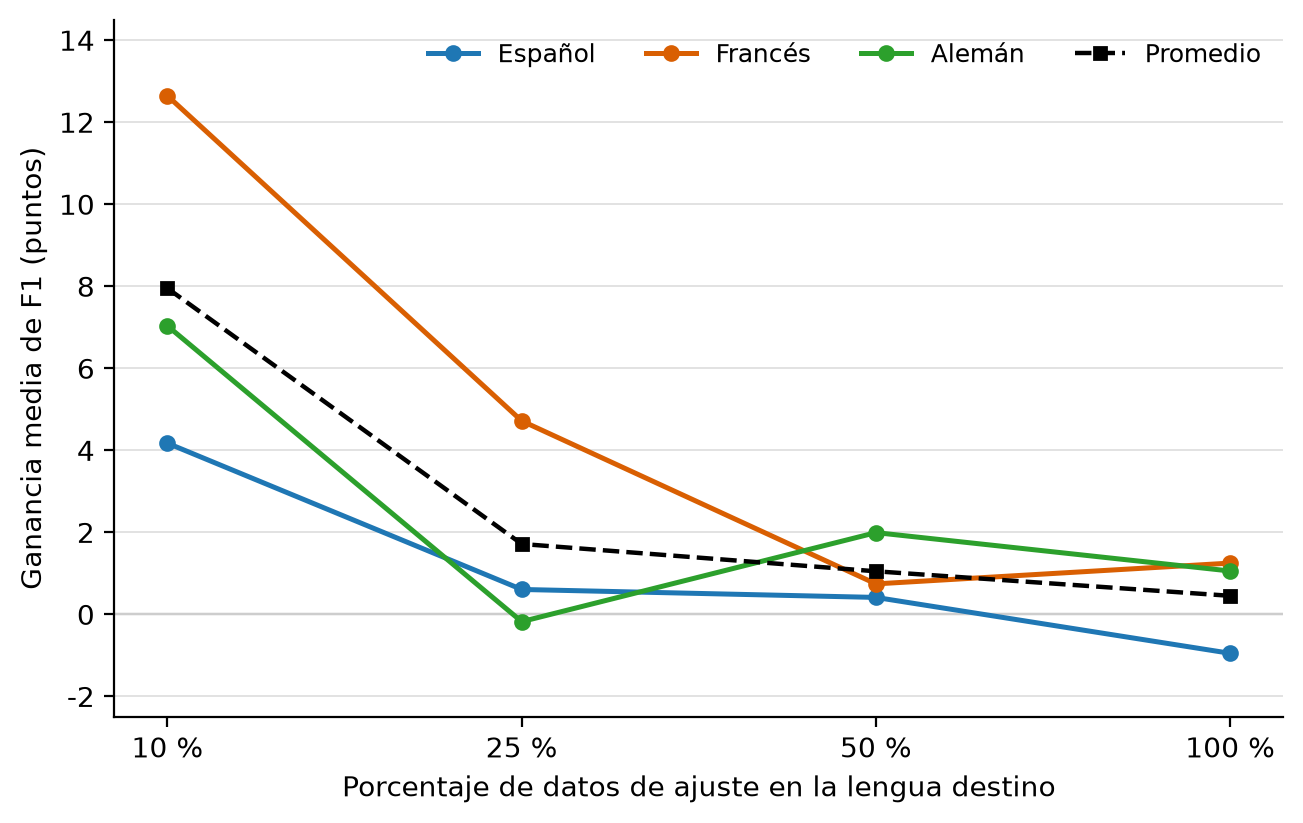
\includegraphics[width=0.78\textwidth]{figuras/ganancia_media.png}
\caption{Ganancia media en puntos de F1 por lengua y tamaño del conjunto de ajuste. Cada punto promedia los tres profesores ($B_p$, $B_{ft}$, $mB_{ft}$) frente a \textit{noKD}; la línea negra promedia las tres lenguas. Elaboración propia a partir de la Tabla~3 de \cite{piperno2025}.}
\label{fig:ganancia}
\end{figure}

El descenso de $+7{,}95$ a $+0{,}45$ tiene una explicación compatible con los datos: el baseline sube. Entre el 10\,\% y el 100\,\%, el noKD sube 16,78 puntos en español, 25,69 en francés y 22,96 en alemán. Cuanto más alto el punto de partida, menos espacio queda para la ganancia. Los autores añaden que la brecha entre BioBERT y mBERT sin destilación en inglés se reduce de unos 10 puntos con el 10\,\% a unos 5 con el 100\,\%. Con pocos datos el profesor aporta la frontera que las etiquetas no definen; con todos, el estudiante la aprende solo.

El ahorro de etiquetas es modesto. El mejor modelo destilado con el 10\,\% no alcanza al noKD con el 25\,\% en ninguna de las tres lenguas: 78,11 frente a 80,46 en español, 76,62 frente a 78,21 en francés y 73,30 frente a 78,34 en alemán. La destilación reduce las etiquetas necesarias, pero no sustituye 15 puntos porcentuales del corpus.

\subsection{Las cinco preguntas}

\textbf{Pregunta 1.} Sí se transfiere, con una precisión: «sin datos en inglés» significa sin etiquetas inglesas en el ajuste final. Con $B_p$, el delta es positivo en 11 de 12 configuraciones; la única excepción es $-0{,}03$ (español, 50\,\%). El conocimiento biomédico se transfiere, aunque el efecto dependa de la lengua y del tamaño de ajuste.

\textbf{Pregunta 2.} También se transfiere, aunque con más celdas negativas. $B_{ft}$ es positivo en 9 de 12 y $mB_{ft}$ en 8 de 12, con un cero. En el 100\,\%, $mB_{ft}$ pierde 1,77 en español y 1,49 en alemán.

\textbf{Pregunta 3.} Los autores no hallan diferencia clara entre $B_{ft}$ y $mB_{ft}$ y concluyen que el mBERT ajustado es más económico. $mB_{ft}$ gana 3 filas, $B_{ft}$ gana 3 y $B_p$ gana 6. Nuestra cautela es que $mB_{ft}$ comparte tokenizador y espacio de embeddings con el estudiante, así que parte de la ganancia podría deberse a esa cercanía.

\textbf{Pregunta 4.} La ganancia media cae de $+7{,}95$ a $+0{,}45$ entre el 10\,\% y el 100\,\%. La supervisión directa reemplaza la señal del profesor.

\textbf{Pregunta 5.} El RSA muestra una correlación de Pearson mayor entre profesor y estudiante después de la destilación, en las tres lenguas y con los tres profesores. Los estudiantes destilados se parecen más entre sí que al noKD. La correlación es más alta con $B_p$ que con los profesores ajustados; los autores lo atribuyen a que el ajuste especializa las capas finales. El RSA es una comprobación del mecanismo, no una prueba de comprensión clínica.

\subsection{MNRL frente a MSE}

MNRL supera a MSE en 32 de los 36 casos, con ventaja mayor cuando hay pocos datos. Los autores lo explican por la sensibilidad de MSE al ruido de la traducción. La comparación tiene dos límites: se reporta de forma gráfica y como conteo, sin tabla por celda, y el artículo presenta el brazo con MSE como reproducción de \cite{reimers2020}, pero la Figura~5 lo aplica a los mismos tres profesores. No se documenta qué se conservó de la receta original, así que la comparación es un cambio de pérdida sobre el flujo propio y no una reproducción verificable.
